\chapter{Higher-Order Regression}

\section{Showing that the Point \texorpdfstring{$(\bar{x}, \bar{y})$}{(x-bar, y
bar)} lies on the Least-Squares Regression Line}
In simple linear regression, the model is given by:
\begin{equation*}
    Y = \beta_0 + \beta_1 x + \epsilon
\end{equation*}
Where:
\begin{itemize}
    \setlength{\itemsep}{-2pt}
    \item $\beta_0$ is the intercept,
    \item $\beta_1$ is the slope, and
    \item $\epsilon$ is the error term.
\end{itemize}
The least squares regression line, which minimizes the sum of squared residuals,
is given by the following equation:
\begin{equation*}
    \hat{Y} = \hat{\beta}_0 + \hat{\beta}_1 x
\end{equation*}
To find the least-squares estimates $\hat{\beta}_0$ and $\hat{\beta}_1$, we have
to minimize the sum of squared residuals (SSR):
\begin{equation*}
\text{SSR} = \sum_{i=1}^{n} \left( y_i - (\hat{\beta}_0 + \hat{\beta}_1 x_i)
\right)^2
\end{equation*}
Partial derivative with respect to $\hat{\beta}_0$:
\begin{equation*}
    \begin{aligned}
        \frac{\partial \text{SSR}}{\partial \hat{\beta}_0} &= -2 \sum_{i=1}^{n}
        \left( y_i - \hat{\beta}_0 - \hat{\beta_1} x_i \right) = 0 \\
        \sum_{i=1}^{n} y_i &= n \hat{\beta}_0 + \hat{\beta}_1 \sum_{i=1}^{n} x_i
        \\
        \hat{\beta}_0 &= \bar{y} - \hat{\beta}_1 \bar{x} \\
    \end{aligned}
\end{equation*}
Partial derivative with respect to $\hat{\beta}_1$:
\begin{equation*}
    \begin{aligned}
        \frac{\partial \text{SSR}}{\partial \hat{\beta}_1} &= -2 \sum_{i=1}^{n}
        x_i \left( y_i - \hat{\beta}_0 - \hat{\beta}_1 x_i \right) = 0 \\
        \sum_{i=1}^{n} x_i y_i &= \hat{\beta_0} \sum_{i=1}^{n} x_i +
        \hat{\beta_1} \sum_{i=1}^{n} x_i^2 \\
        \hat{\beta_1} &= \frac{\sum_{i=1}^{n} (x_i - \bar{x})(y_i - \bar{y})}
        {\sum_{i=1}^{n} (x_i - \bar{x})^2} \\
    \end{aligned}
\end{equation*}
Now, substituting $\bar{x}$ into the regression line equation gives
\begin{equation*}
\hat{Y} = \hat{\beta}_0 + \hat{\beta}_1 \bar{x}
\end{equation*}
Substitute $\hat{\beta}_0 = \bar{y} - \hat{\beta}_1 \bar{x}$:
\begin{equation*}
\hat{Y} = (\bar{y} - \hat{\beta}_1 \bar{x}) + \hat{\beta}_1 \bar{x}
\end{equation*}
Simplifying this:
\begin{equation*}
    \hat{Y} = \bar{y}
\end{equation*}
Thus, the point $(\bar{x}, \bar{y})$ lies exactly on the least-squares regression
line.

\section{New model using \texorpdfstring{$z = x - \bar{x}$}{z = x - x-bar}}

The original least-squares estimate for $\beta_1$:

\begin{equation*}
    \hat{\beta}_1 = \frac{\sum (x_i - \bar{x})(y_i - \bar{y})}{\sum (x_i -\
    \bar{x})^2}
\end{equation*}
Since $z_i = x_i - \bar{x}$, this can be rewritten in terms of $z$:

\begin{equation*}
    \hat{\beta}_1^* = \frac{\sum z_i (y_i - \bar{y})}{\sum z_i^2}
\end{equation*}
The original least squares estimate for $\beta_0$:

\begin{equation*}
    \hat{\beta}_0 = \bar{y} - \hat{\beta}_1\bar{x}
\end{equation*}
For the intercept in the new model, we know that $z$ is centered around 0,
which means $\bar{z} = 0$. Therefore, the least squares estimate of $\beta_0^*$
is simply the average of $y$, i.e., $\bar{y}$:

\begin{equation*}
    \hat{\beta}_0^* = \bar{y}
\end{equation*}
Since $z = x - \bar{x}$, this is just a change in the predictor variable.
Therefore, the slope of the regression line does not change, and we have the
following:

\begin{equation*}
\hat{\beta}_1^* = \hat{\beta}_1
\end{equation*}
In the new model, the least squares estimates of $\beta_0$ are:

\begin{equation*}
\hat{\beta}_0^* = \bar{y}
\end{equation*}
On the other hand, in the original model, the least squares estimate of $\beta_0$
is:

\begin{equation*}
\hat{\beta}_0 = \bar{y} - \hat{\beta}_1 \bar{x}
\end{equation*}
Thus, the relationship between $\beta_0$ and $\beta_0^*$ is:

\begin{equation*}
\hat{\beta}_0^* = \hat{\beta}_0 + \hat{\beta}_1 \bar{x}
\end{equation*}

\noindent \textbf{Model Differences:}
The original model estimates both the intercept and slope based on uncentered
values of $x$, while the transformed model estimates the intercept at the mean of
$Y$ and uses a centered version of $x$ (now $z$). The slope remains the same in
both models.

\noindent \textbf{Interpretation Differences:}
The intercept in the original model reflects the value of $Y$ when $x$ is zero
(or of a different origin), while in the new model, it represents the mean of
$Y$ at the mean of $x$, providing a different baseline from which predictions are
made.

\section{Regression for a Dataset}

\begin{figure}[H]
  \centering
  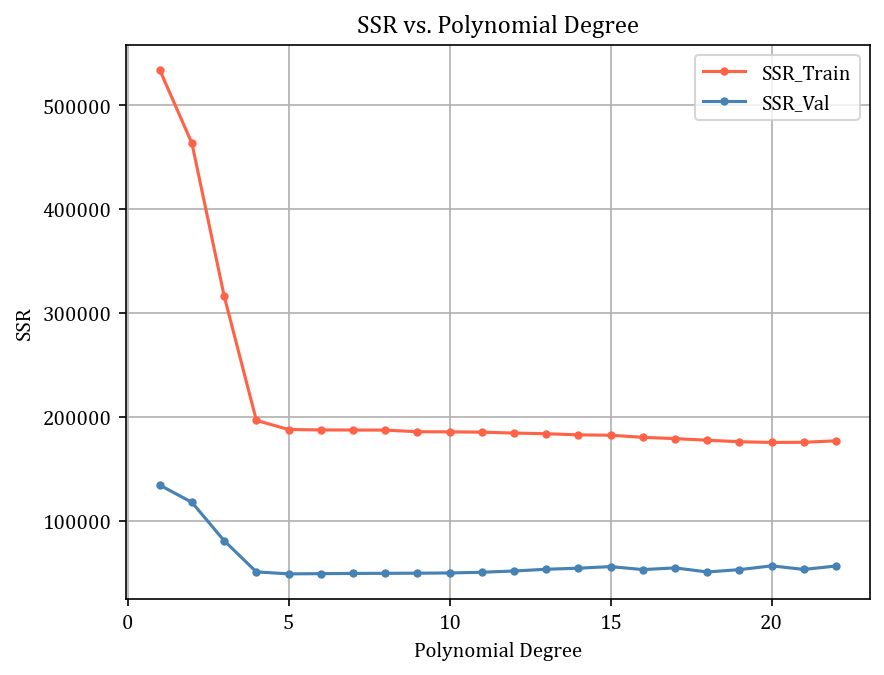
\includegraphics[width=0.3\textwidth]{assets/images/SSR-graph.png}
  \caption{The SSR graph for various degrees}
\end{figure}

By the SSR graph above, degree = 5 seems to be the optimal degree for the
polynomial.

\subsection{Correct Fit}
\begin{figure}[H]
  \centering
  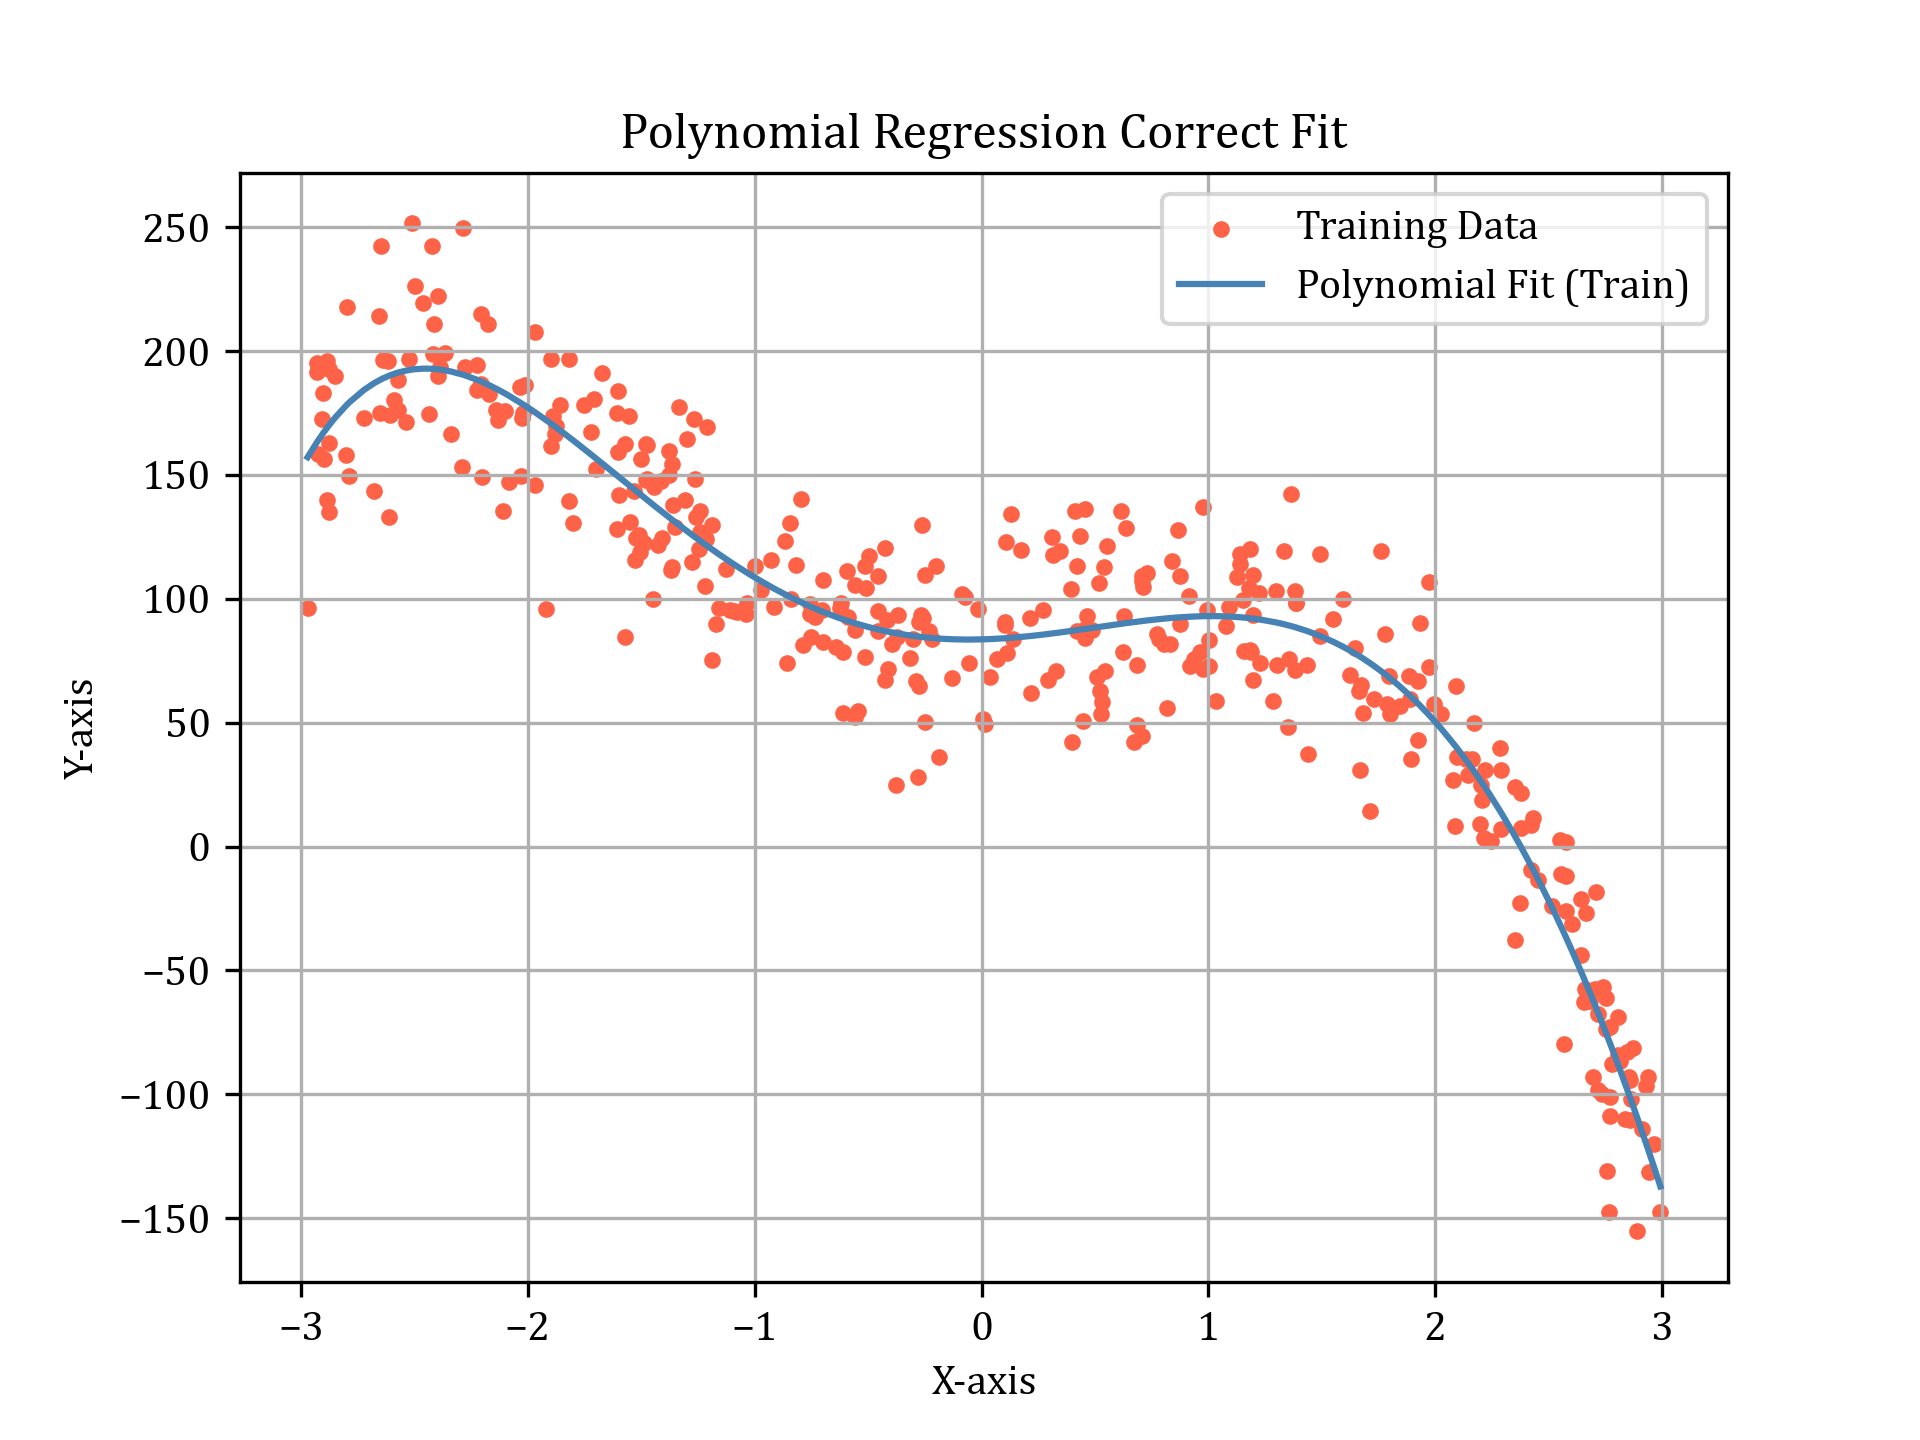
\includegraphics[width=0.4\textwidth]{assets/images/3_correctfit.png}
  \caption{Correct Fit at degree = 5}
\end{figure}

\subsection{UnderFit}
\begin{figure}[H]
  \centering
  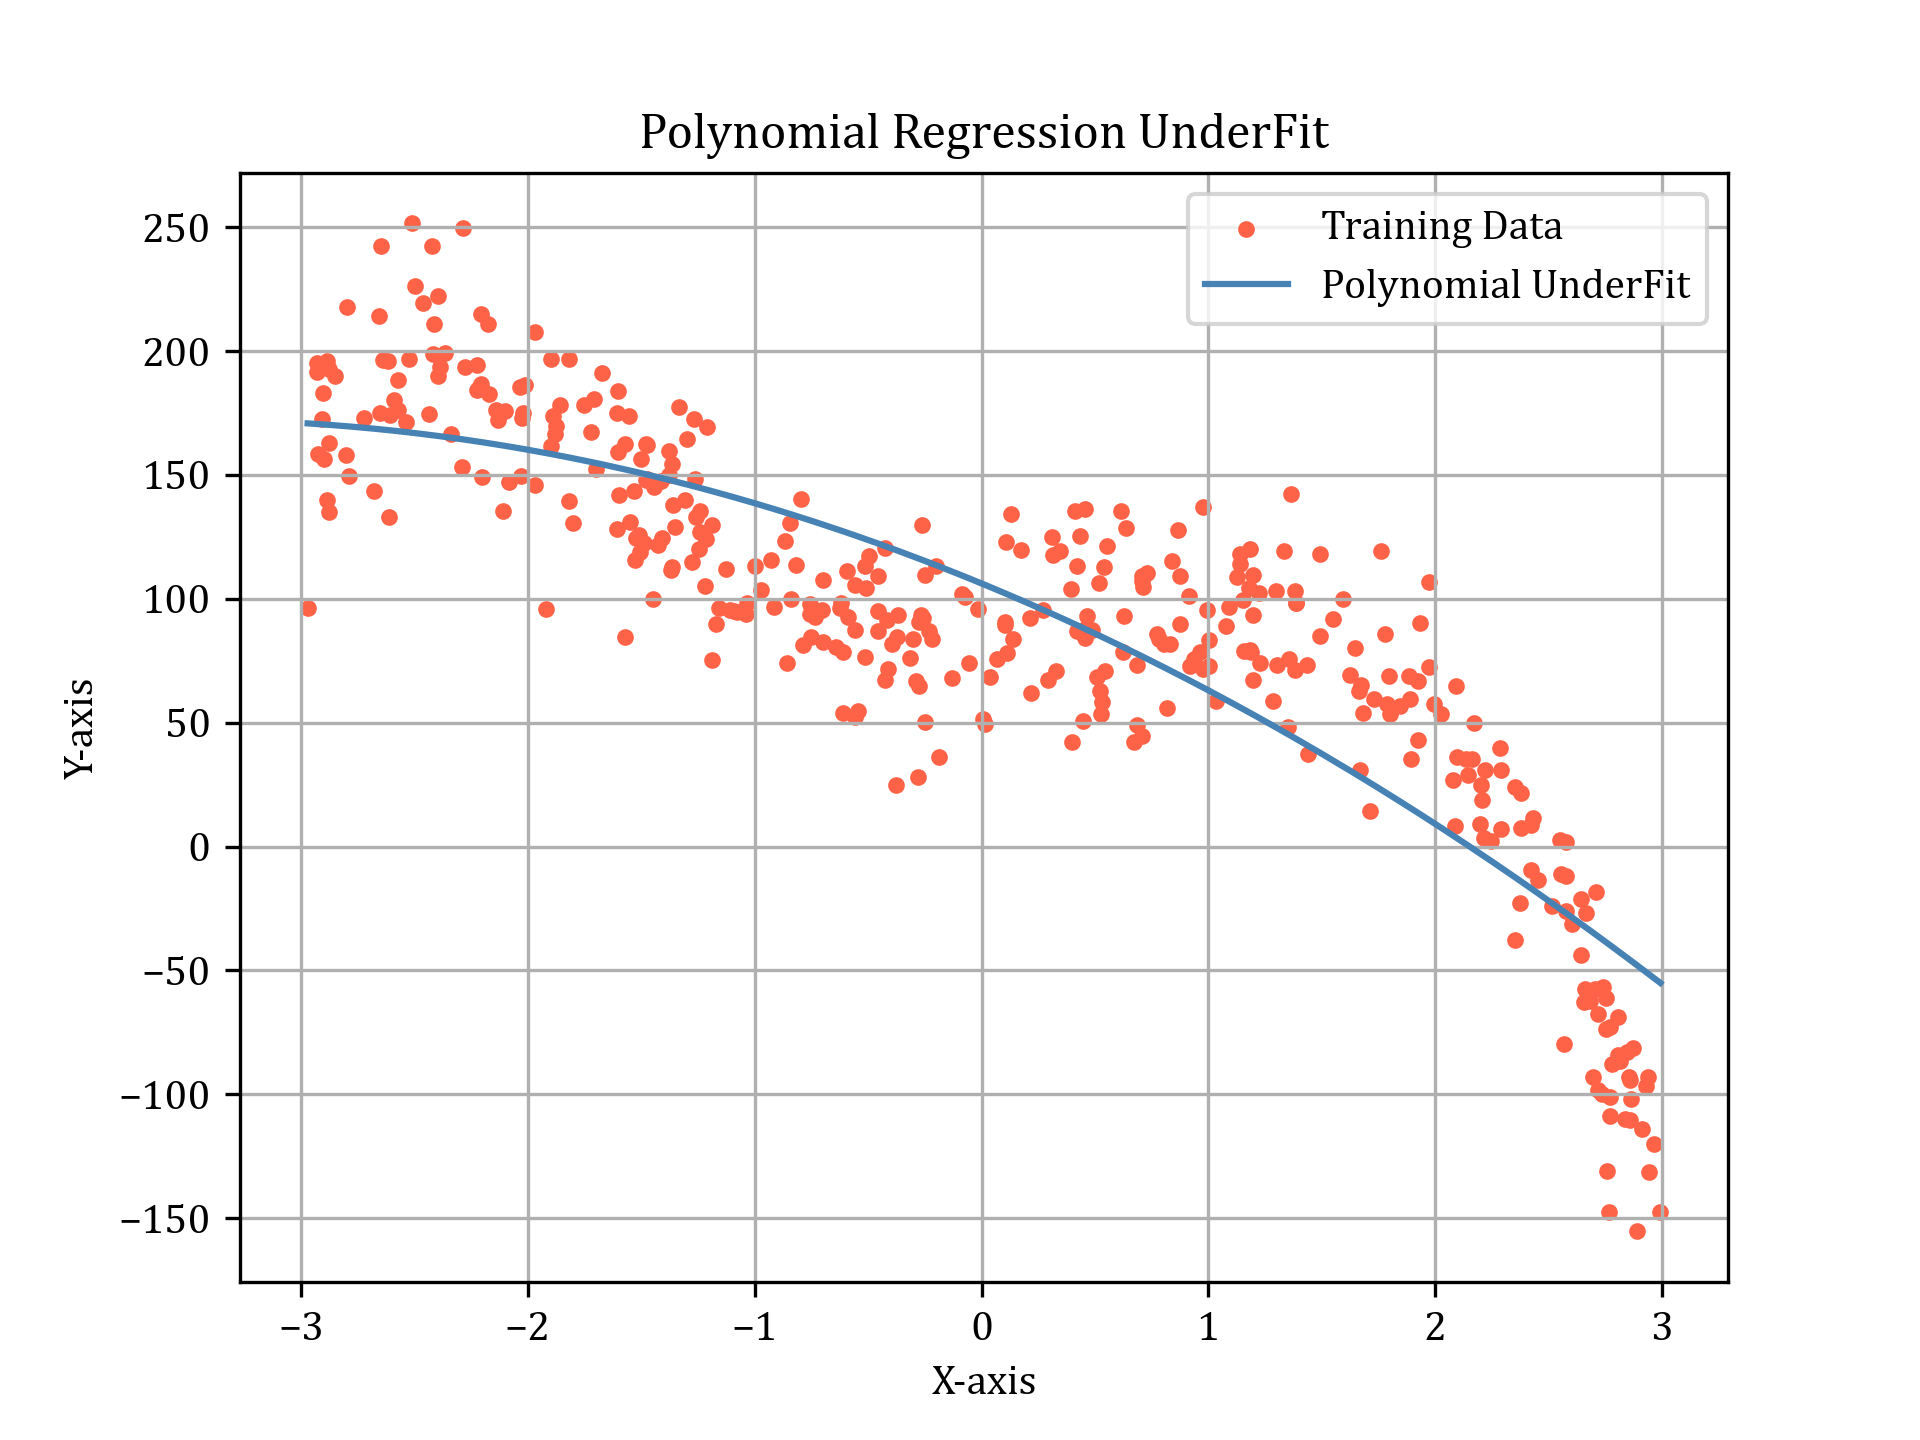
\includegraphics[width=0.4\textwidth]{assets/images/3_underfit.png}
  \caption{UnderFit at degree = 2}
\end{figure}

\subsection{OverFit}
\begin{figure}[H]
  \centering
  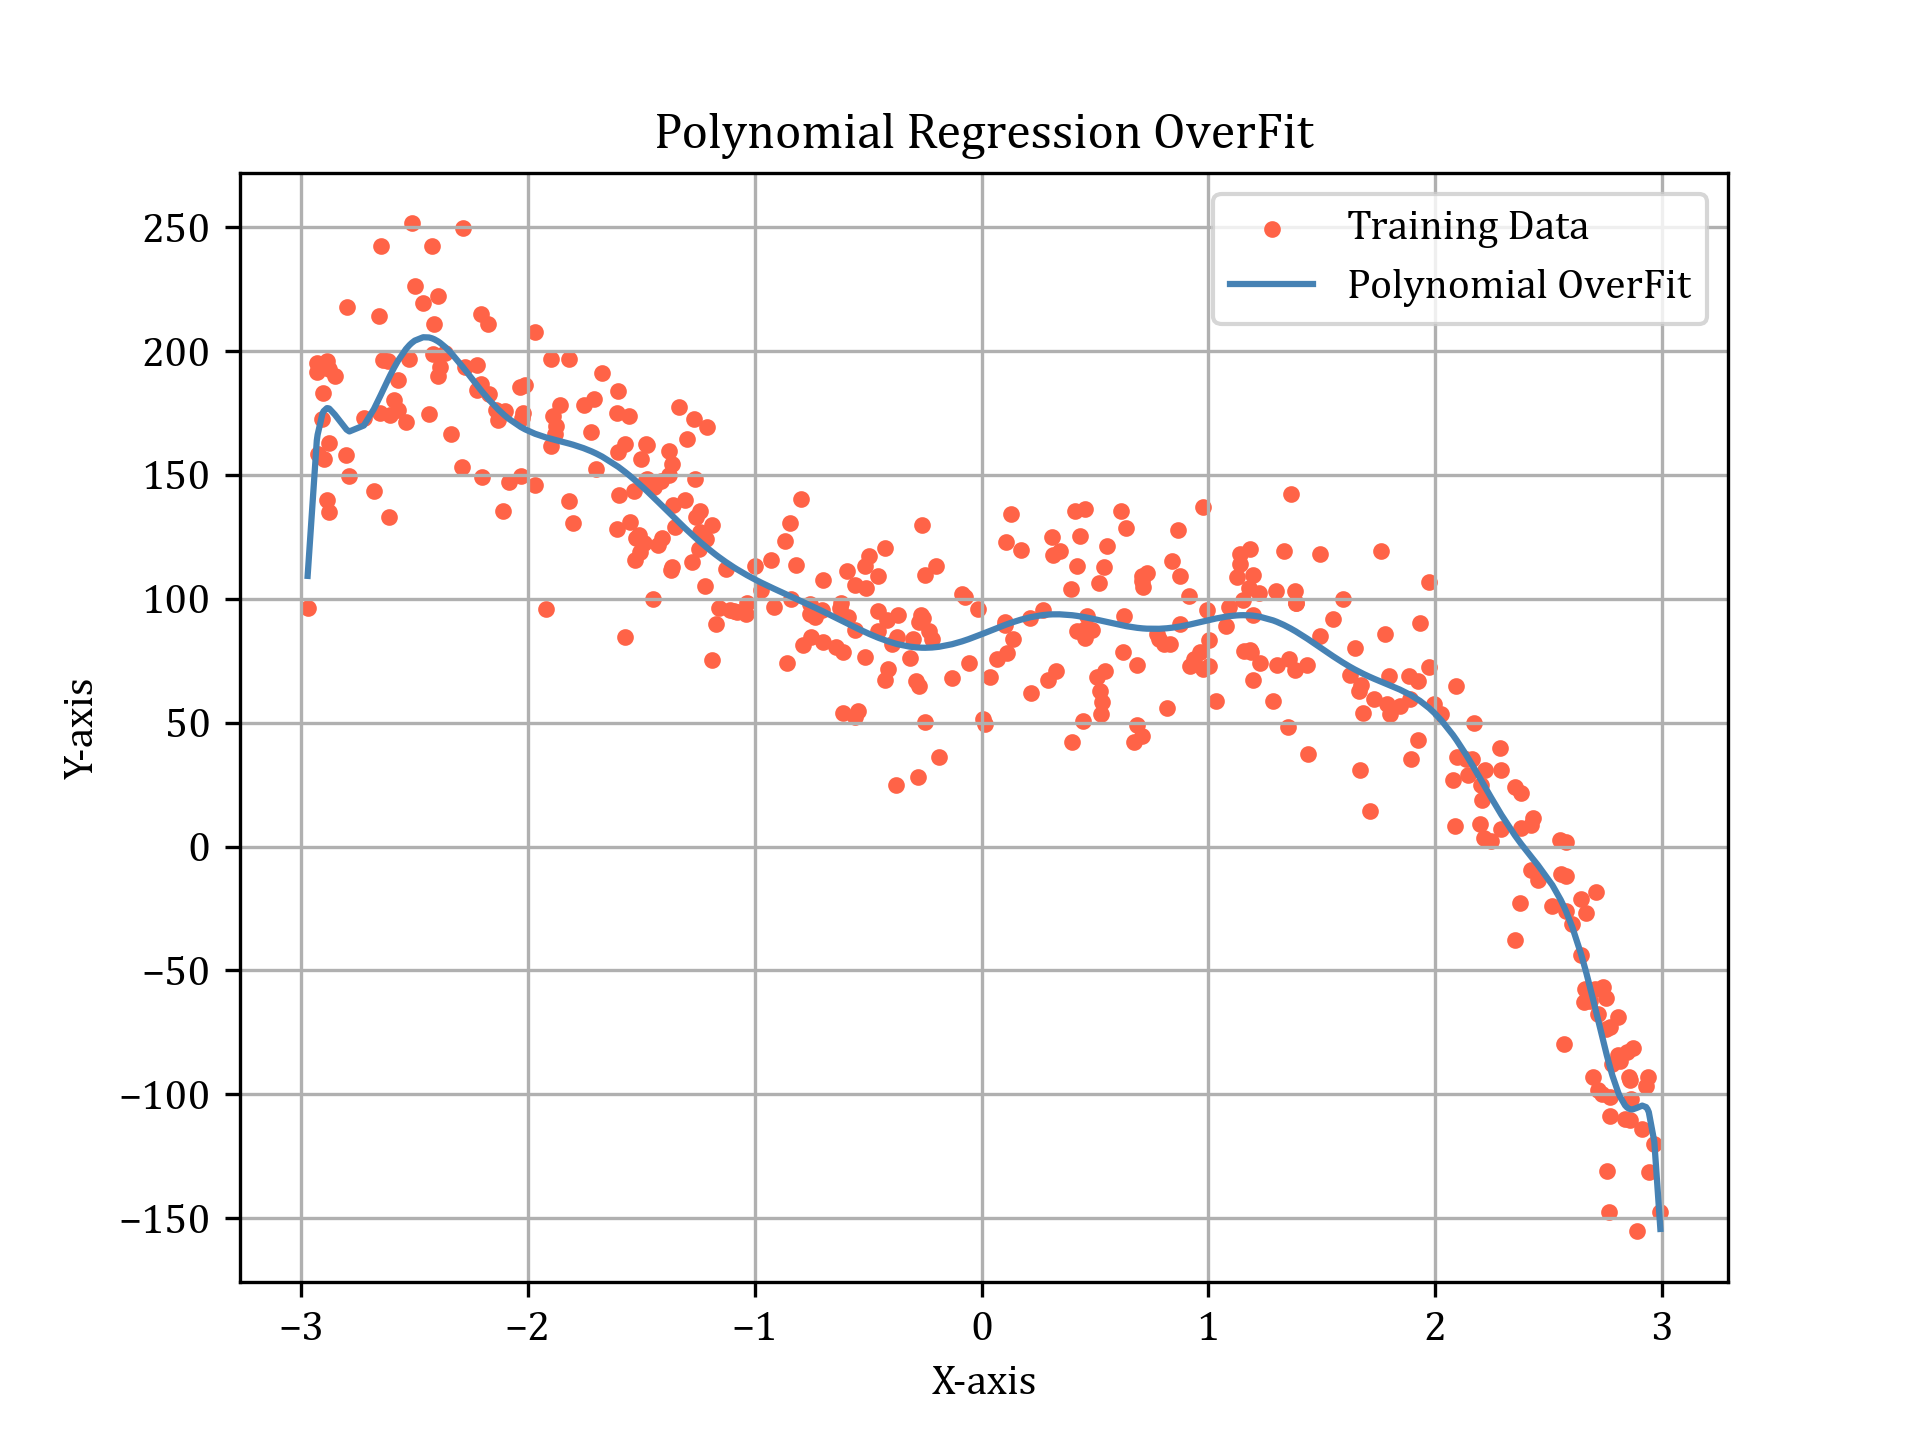
\includegraphics[width=0.4\textwidth]{assets/images/3_overfit.png}
  \caption{OverFit at degree = 20}
\end{figure}
